%
% $Id: ch01_overview
%
%   *******************************************************************
%   * SEE THE MAIN FILE "AllegThesis.tex" FOR MORE INFORMATION.       *
%   *******************************************************************

\chapter{Introduction}
\label{ch:intro}

In the early days of computing, real-time rendering engines that powered games like ``Doom'' or ``NetHack'' had to run on extremely underpowered hardware and render on low-resolution screens.
The dream of real-time, photorealistic graphics was far, far away.
However, even then the simple, blocky graphics, easily recognizable shapes, and maze-like environments were fantastic entertainment.
Today the retro-style of low-resolution graphics, pixel art, and 8-bit color abounds in the gaming space.
\name\ is one part of enabling that retro-aesthetic to grow into a new and unique style that, while similar to the old classics, can be more engaging and real than they ever were.

This thesis document describes a system that creates a moving image on a terminal screen.
This system is called \name; it performs real-time updating of the displayed image, thus generating a window into a three-dimensional (3D) world.
\name\ is available for a wide variety of other programs to use as a rendering engine.
With the current generation of powerful computers, able to execute billions or even trillions of calculations per second, it is finally possible to do real-time, close-to-photorealistic rendering.
While the goal of \name\ is not high-resolution photorealism, some approximation is achieved.

In this introduction to \name, we will first cover the motivations behind creating this system in Section~\ref{ch:intro:motivation}.
Then, we will give an overview of the project in Section~\ref{ch:intro:overview}.
Section~\ref{ch:intro:background} expands on the overview to provide some mathematical grounding for some of the algorithms used in \name.
In Section~\ref{ch:intro:background:development_ecosystem} we cover the main development tools used in this project, such as the implementation language.
Finally, Section~\ref{ch:intro:outline} outlines the rest of this thesis document, introducing the major topics of discussion for the remaining chapters.

\section{Motivation}
\label{ch:intro:motivation}

I have always been fascinated with rendering algorithms, especially ray-tracing.
This fascination fueled an interest in game engine development, 3D modeling, and other computer graphics topics.
The idea for \name\ came out of a disappointment -- I was working on a project that made a virtual space seem larger than it was when the user was wearing a virtual reality headset.
Sadly, someone had already developed a toolkit that did exactly what I wanted to achieve.

Through my search for a replacement project, I discovered that, for me, one of the biggest draws to an idea was the ability for that idea to affect other people.
Whether it was something that many others could use or an idea that people could contribute to, I wanted to make something other people saw.
That is where the draw of open-source software came from for me, and why \name\ is open-source.
Additionally, I discovered that there are many niches in software -- places where there just is not a lot of people making things.
Computer graphics in a terminal emulator (see Section~\ref{ch:intro:overview:libtickit}) is one of those corners.
The only real application many people saw for this niche was the rendering of images to the terminal -- in fact, some of the initial inspiration for \name\ came from TerminalImageViewer \cite{tivGithub}, a program to accomplish that very task.

I saw more possibilities, however.
There is no need to keep the terminal in a by-gone era, stuck with only colored characters and still graphics.
The terminal is, after all, only a window into some text.
Why does this text have to be stationary?
Why does it need to be text at all?
The answer, of course, is that it does not.
There is a huge amount of potential in a 3D rendering engine that outputs to the terminal -- there are so many applications, from rendering 3D model files to playing video games to visualizing music.
All that these programs need is an infrastructure around the terminal for 3D rendering.
\name\ aims to create that infrastructure through a completely novel combination of ray-traced 3D rendering and Unicode-based image composition.

\section{Overview}
\label{ch:intro:overview}

\name\ uses the recursive ray-tracing algorithm, simulating the path of light through the scene -- this is described in more detail in Section~\ref{ch:intro:overview:raytracing}.
Many images are generated, or rendered, each second; once an image is rendered the Tickit library \cite{libtickitLibrary} is used to display it in a terminal.
Multiple images are displayed in quick succession, creating the illusion of movement.
More details on this process are given in Section~\ref{ch:intro:overview:libtickit}.
Rendered images are displayed in two different modes; the first uses single half-character pixels, and the second more complex Unicode block characters.
The mechanics of these image composition methods are discussed in Section~\ref{ch:intro:overview:unicode}.
Finally, Figure~\ref{fig:checker_metal} is a still image of the final terminal output \inlinetodo{update with actual output image}.

\begin{figure}[htb]
  \centering
  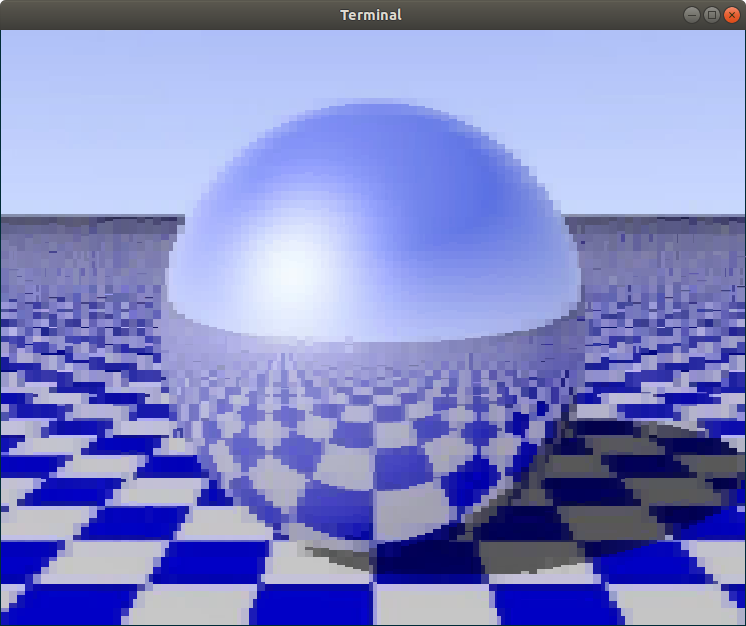
\includegraphics[width=0.8\textwidth]{resources/checker_metal}
  \caption{Example of terminal output}
  \label{fig:checker_metal}
\end{figure}

\subsection{Rendering Engines and Ray-Tracing}
\label{ch:intro:overview:raytracing}

A rendering engine is an algorithm that takes a scene -- a description of some collection of objects -- and generates an image or visual representation of that scene.
There are many different algorithms that accomplish this goal.
\name\ utilizes a variant of the recursive ray-tracing algorithm first pioneered by Turner Whitted in his ground-breaking paper ``An Improved Illumination Model for Shaded Display'' \cite{whitted1980improved}.
Ray-tracing was one of the first algorithms developed in the field of computer graphics, and although there have been some improvements since then, the idea behind the algorithm has maintained its original simplicity.

Ray-tracing has been used as the rendering algorithm of choice for photorealistic scenes because with only a few modifications to Whitted's original algorithm, it can generate fantastic images.
In the past, however, render times have been so slow that it was impossible to generate images fast enough for real-time use.
For example, Figure~\ref{fig:povray_render} is a render created by the POV-Ray engine \cite{povray}.
POV-Ray can take between a few minutes to several hours to complete one single image depending on the processing power involved.
However, there have been a few recent innovations that change this, such as NVIDIA's RTX hardware acceleration.
Section~\ref{ch:intro:background:hardware} provides more details on these advances and how \name\ takes advantage of them.

\begin{figure}[htb]
  \centering
  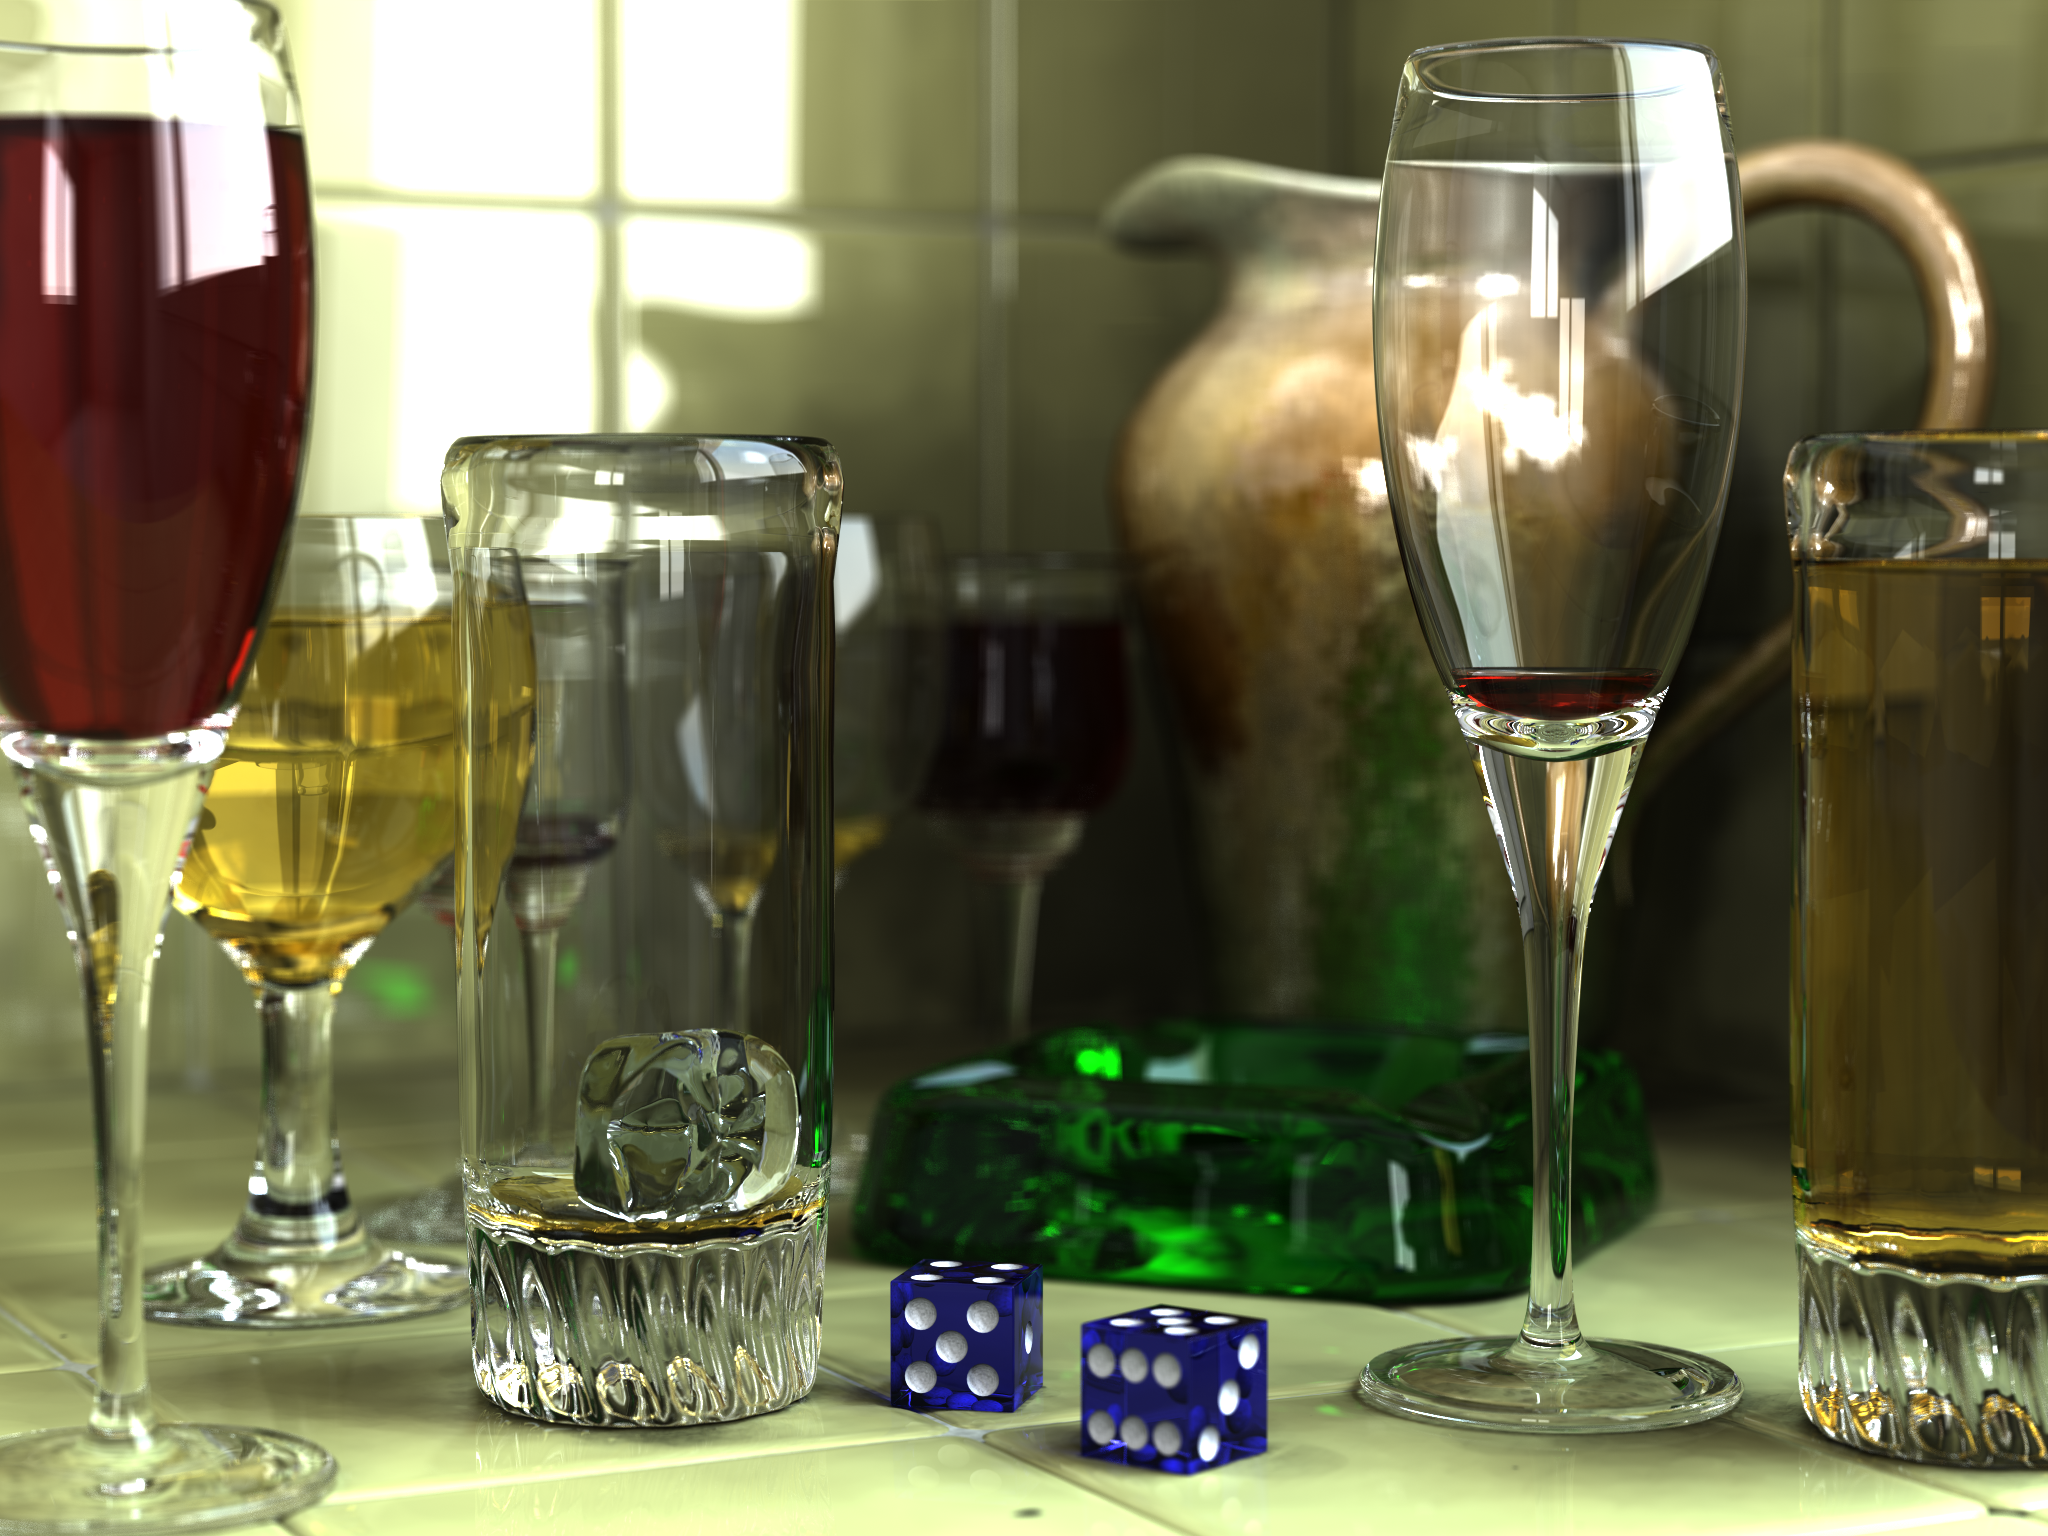
\includegraphics[width=0.8\textwidth]{resources/glasses_povray}
  \caption{POV-Ray render created by Gilles Tran \cite{povray2006render}}
  \label{fig:povray_render}
\end{figure}

Ray-tracing revolves around the idea of {\it rays}, a mathematical construct that represents an infinite line emanating in some direction from a starting point in three-dimensional space.
In \name\, rays are used to simulate the path that light takes as it travels around the scene.
When a ray intersects with an object in the scene various interactions take place that simulate how light may travel under different conditions.
It is worth noting that a base assumption is made in ray-tracing when using straight rays as described here: light follows a straight line without changes.
This is only the case in reality when light travels through a vacuum with no gravitational bodies; thus, basic ray-tracing is not exactly photorealistic and does not model phenomena like atmospheric scattering.
Additional mathematics and systems must be used to bend, attenuate, or scatter a ray to accurately render transparent volumes -- this is called volumetric ray-tracing.
Volumetric ray-tracing is not currently supported in \name, but is a fascinating area for future work.

The formal basis for ray-tracing is the rendering equation, articulated by James Kajiya in 1986 \cite{kajiya1986rendering}.
The rendering equation models the outgoing light at some point in some direction given all incoming light, a bidirectional reflectance distribution function (BDRF), and a normal (a perpendicular direction) for the surface at the point modeled.
If solved for every point in the scene, the rendering equation could generate a completely photorealistic image -- this would, however, require massive amounts of computation.
This is because the rendering equation contains an integral over all incoming light which must be solved through numerical analysis.
Ray-tracing algorithms that do this are known as {\it path-tracers} and are the most photorealistic rendering algorithms invented.

\name\ does not use a full path-tracer -- such algorithms are still many times too slow for most real-time rendering situations; however, a Monte-Carlo method that can approximate a full path-tracer is used.
In \name, the rendering equation is solved by sampling the incoming light at each point with rays.
This is known as recursive ray-tracing since it starts with a single ray that ``recurses'' when it encounters a surface.
The eventual goal of the recursive ray-tracing algorithm is to create a tree of rays for each {\it fragment} to render.
A fragment is either a pixel or some sub-pixel -- many systems will use many fragments per pixel to get better anti-aliasing and more accurate results.
Each ray contains some color that represents the color of the light in that ray.
When a ray hits an object, it is {\it scattered} by the {\it material} of the object, generating a new ray.
This ray's trajectory is modified randomly based on probability and the specific material hit; for instance, if the material is reflective then the ray will be biased towards the reflection direction.

The base of each generated tree is an {\it eye-ray} -- a ray with its origin at the fragment location on the camera plane.
The eye-ray's color is the color that will be rendered for that fragment.
As the eye-ray projects forward, away from the eye, it is tested for intersection with all objects in the scene.
When an intersection happens and the generated rays scattered, the eventual color values of the scattered rays are combined to produce the color of the original eye-ray.
This is done recursively to fully render the scene.

\subsection{Terminal Output using Tickit}
\label{ch:intro:overview:libtickit}

Output in \name\ is shown in a terminal window.
A terminal is a specific kind of interface for a computer that uses text-based commands and feedback, as opposed to a Graphical User Interface (GUI).
It descends from the old days of mainframe computers, where the actual computer was not under a desk -- instead, users would connect over a network to the main computer, using an actual terminal machine.
Today, the terminals most people use are actually ``terminal emulators'', because they simply emulate these old mainframe terminal machines.
These terminal emulators are often simply programs that run in an existing graphical desktop environment, providing a text-based interface to the operating system.

Once an image is generated, \name\ must somehow display that image in a terminal with no surrounding prompt or other formatting -- as a simple {\it character field}.
To do this, we use a two-step approach: first, we represent the image using Unicode characters (see Section~\ref{ch:intro:overview:unicode}), then we print those characters to the terminal using the Tickit (Terminal Interface Construction Kit) library \cite{libtickitLibrary}.
This library abstracts implementation details of the terminal to enable full-window 24-bit color character output.
In \name, the terminal window is divided into two ``panels'', a main panel for the actual image output -- updated 30 times or more per second -- and an info panel to render information such as frames per second and logging text.
Additionally, extra terminal output such as the command prompt or other character output is disabled.

The main problems that Tickit solves are ones which need to use terminal escape codes -- short character sequences that tell a terminal emulator to change some specific data or use a different display method.
These escape codes tell the terminal how to display text by changing the formatting, positioning, or color.
The library also disables character ``echoing'', the display of characters that are typed by the user.
Because of this dependency on Tickit, \name\ can be used only with terminals that support it -- generally, any XTerm-like terminal will work, as long as it supports \texttt{terminfo} \cite{libtickitLibrary}.
Additionally, full RGB direct color support is required for accurate color information.

\subsection{Image Composition using Unicode Characters}
\label{ch:intro:overview:unicode}

Unicode is a character standard that allows anyone to reference many thousands of characters to compose text, no matter the environment around the text \cite{unicode}.
Some critical characters that \name\ uses are known as the {\it block characters} -- they are characters \texttt{U+2580} -- \texttt{U+259F}, a subset of which are shown in Figure~\ref{fig:unicode_characters}.
The core of image composition using Unicode is an algorithm coloring the characters and the background -- \name\ uses this algorithm on every character of the output to both determine the character to display, and the foreground and background colors for that character.
The foreground colors the character itself, whereas the background provides a relief color.
This allows each {\it character~pixel} to represent a hard gradient.

\begin{figure}[htb]
  \centering
  \hspace{0.3em}
  \begin{subfigure}[htb]{0.4\textwidth}
    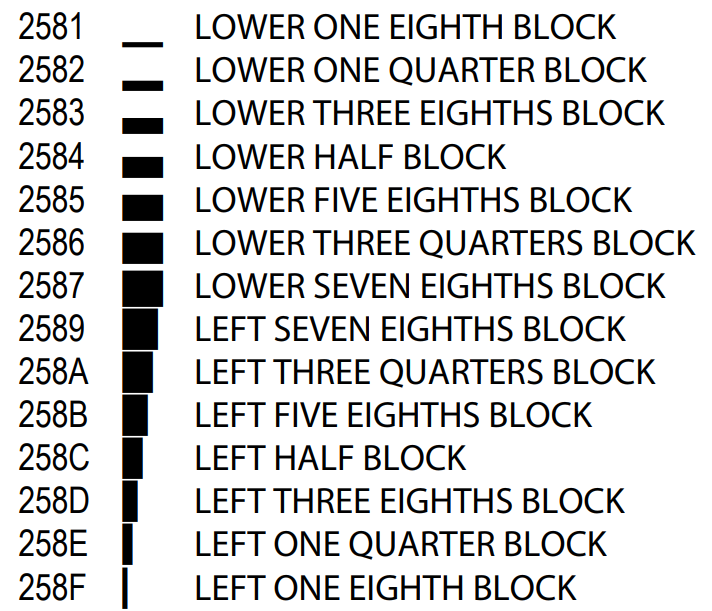
\includegraphics[width=\textwidth]{resources/block_elements}
    \caption{Block Elements}
    \label{fig:unicode_block_characters}
  \end{subfigure}
  \hfill
  \begin{subfigure}[htb]{0.51\textwidth}
    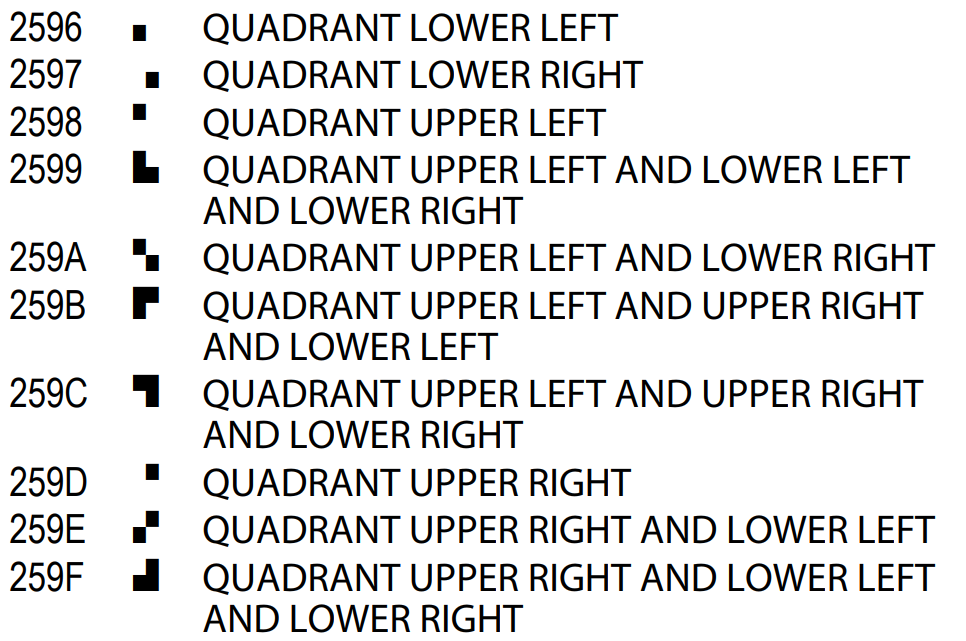
\includegraphics[width=\textwidth]{resources/quadrant_elements}
    \caption{Quadrant Elements}
    \label{fig:unicode_quadrant_characters}
  \end{subfigure}
  \caption{Subset of \texttt{U+2580} -- \texttt{U+259F} \cite{unicode}}
  \label{fig:unicode_characters}
\end{figure}

There are two main image modes possible for use in \name.
The first is pure {\it pixel mode}, in which the Unicode ``half-block'' symbol (\texttt{U+2584}) is used; this is the current default.
Since monospaced character output (such as in a terminal) is twice as tall as it is wide, the half-block can split a single character into two pixels that are colored differently: the upper pixel with the background color of the character, and the lower with the character or foreground color of the pixel.
This means that a typical 85 by 30 character terminal results in a screen space of 85 by 60 pixels.
This mode also dramatically reduces the number of ray-tracing computations needed, since only one ray per pixel per sample is required.

The second image mode is considerably more complicated and slower, as it uses significantly more rays per character in order to determine what Unicode block character most fits the desired output.
On the other hand, it allows a much higher perceived resolution, since the characters used have smaller footprints of down to an eighth of a character in width or length.
The differences between these two modes are highlighted in Figure~\ref{fig:unicode_mode_comparison1} and~\ref{fig:unicode_mode_comparison2}.
It can be seen that the first image mode, {\it pixel mode}, shows a rather fuzzy definition of the main large sphere.
However, in the second image mode, {\it character mode}, the sphere and the reflections seen in it are more defined.
The performance impact of both modes is another factor that is assessed when making implementation decisions for \name; it informed how much actual definition was added by the second rendering mode.
The current implementation does not fully implement character mode; instead, this is considered a well-defined area for future work.

\begin{figure}[htb]
  \centering
  \begin{subfigure}[htb]{0.49\textwidth}
    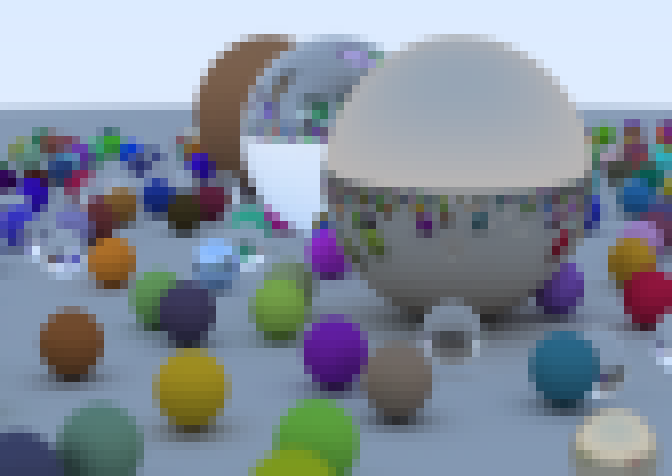
\includegraphics[width=\textwidth]{resources/many_spheres_square}
    \caption{Pixel Mode Image Output}
    \label{fig:unicode_mode_comparison1}
  \end{subfigure}
  \hfill
  \begin{subfigure}[htb]{0.49\textwidth}
    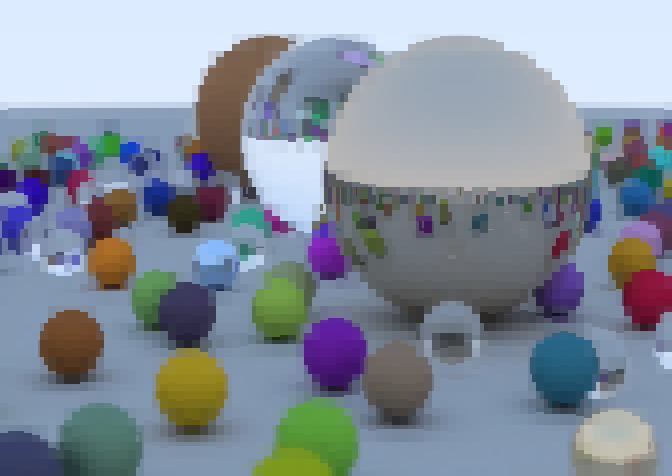
\includegraphics[width=\textwidth]{resources/many_spheres}
    \caption{Character Mode Image Output}
    \label{fig:unicode_mode_comparison2}
  \end{subfigure}
  \caption{Examples of Image Mode Output}
  \label{fig:unicode_mode_comparison}
\end{figure}

\section{Background}
\label{ch:intro:background}

The background information for the algorithms and techniques used to implement \name\ is discussed in this section.
We introduce basic vector mathematics in Section~\ref{ch:intro:background:vector_math}.
In Section~\ref{ch:intro:background:raytracing_math} we detail most of the specific mathematical algorithms involved.
In \name, many of these algorithms are implemented behind the scene in APIs like OptiX and CUDA \inlinetodo{update with actual implementation location}.

\subsection{Vector Mathematics}
\label{ch:intro:background:vector_math}

Vector mathematics is a way to represent operations on $n$-dimensional constructions.
The main unit of computation is a vector -- essentially, a list of $n$ numbers.
A vector is denoted with an arrow over its name: $\vec{v} = (-2, 3, 1)$ is a vector.
A specific value in a vector is referenced by either its zero-based index, $\vec{v}_{0}$ is the first value in $\vec{v}$ (note the arrow is above $v$ only, and not the index), or its dimension -- $\vec{v}_x$ is the same value.
The dimensions are by convention $x$, $y$, $z$, and $w$.
In \name\ however, we generally work only with vectors where $n = 3$ (only in $x$, $y$, and $z$), and each vector represents either a direction or a position in three-dimensional space.
Vectors are related to both multivariable calculus and linear algebra -- an expansion on this basic explanation can be found in virtually any textbook on these topics.

\littlesection{Vector Operations}

Each set of all possible $n$-dimensional vectors are closed under the basic arithmetic operations.
Addition, subtraction, along with some specialized versions of multiplication, are all defined.
Addition and subtraction are calculated on a component-wise basis -- for instance, in three dimensions addition and subtraction can be calculated using Formulas \ref{equation:vector_addition} and \ref{equation:vector_subtraction}.

\begin{equation}
  \label{equation:vector_addition}
  \vec{u} + \vec{v} = (\vec{u}_x + \vec{v}_x, \vec{u}_y + \vec{v}_y, \vec{u}_z + \vec{v}_z)
\end{equation}

\begin{equation}
  \label{equation:vector_subtraction}
  \vec{u} - \vec{v} = (\vec{u}_x - \vec{v}_x, \vec{u}_y - \vec{v}_y, \vec{u}_z - \vec{v}_z)
\end{equation}

There are three other operations, each based on numerical multiplication.
The first is simple scalar multiplication.
A scalar in this context is just a regular number, such as $2$.
Scalar multiplication is defined by Formula~\ref{equation:vector_scalar_multiplication}, and is also a closed operation for $n$-dimensional vectors.

\begin{equation}
  \label{equation:vector_scalar_multiplication}
  k\vec{v} = (k\vec{v}_x, k\vec{v}_y, k\vec{v}_z)
\end{equation}

Then we have the cross product.
This is a specialized multiplication operation only applicable when $n = 3$ that results in a vector that is perpendicular to both of its operands.
The cross product of $\vec{u}$ and $\vec{v}$ is denoted as $\vec{u} \times \vec{v}$, and can be calculated with Formula~\ref{equation:vector_cross_product}.

\begin{equation}
  \label{equation:vector_cross_product}
  \vec{u} \times \vec{v} = (\vec{u}_y\vec{v}_z - \vec{u}_z\vec{v}_y, \vec{u}_z\vec{v}_x - \vec{u}_x\vec{v}_z, \vec{u}_x\vec{v}_y - \vec{u}_y\vec{v}_x)
\end{equation}

Finally, the dot product is a third multiplication operation that is applicable to any $n$-dimensional vector.
However, the result of the dot product operation is a simple scalar, not a new vector.
The dot product only makes semantic sense when talking about direction vectors: it gives a sense of how much two vectors are ``aligned'' with each other.
It is often used to determine if two vectors are at right angles with each other, since in that case the dot product would be $0$.
The dot product of $\vec{u}$ and $\vec{v}$ is denoted as $\vec{u} \bullet \vec{v}$, and can be found using Formula~\ref{equation:vector_dot_product}.

\begin{equation}
  \label{equation:vector_dot_product}
  \vec{u} \bullet \vec{v} = \vec{u}_x\vec{v}_x + \vec{u}_y\vec{v}_y + \vec{u}_z\vec{v}_z
\end{equation}

\littlesection{Vector Equations}

With the operations described above, we can write equations using vectors.
This greatly simplifies the description of the mathematics in Section~\ref{ch:intro:background:raytracing_math}, since without vector mathematics every operation would need to be notated in cartesian coordinates.
It should be noted that exponentiation for vectors is calculated on a component-wise basis -- for example, $\vec{(1, 4, 2)}$ squared is $\vec{(1, 16, 4)}$.
This is by convention in graphics programming since it provides an easy description of such an operation.
This is not, however, always the case in other mathematical applications of vectors.

When thinking about the meaning and algorithms behind equations, it is extremely helpful to keep two main facts in mind.
First, {\it crossing} two vectors results in a vector that is at a right angle to each; that is, it gives a normal to the plane in which both original vectors lie.
We should note here that according to only this definition, there are actually two possible answers for each set of operands.
However, only one of these answers is correct; to determine the right one, the ``right-hand rule'' is used.
To use the right-hand rule, point your right hand's index finger in the direction of the first vector, and your middle finger in the direction of the second.
Your thumb will point in the direction of the resulting cross product.
Note that this causes the order of operands to matter -- a different order will produce the opposite direction.

\begin{equation}
  \label{equation:vector_dot_product_cos}
  \vec{u} \bullet \vec{v} = |\vec{u}| \cdot |\vec{v}| \cdot cos(\theta)
\end{equation}

Second, {\it dotting} two vectors multiplies their lengths while keeping in mind their direction -- two vectors perfectly parrallel to each other would have a dot product that was simply their lengths multiplied.
However, two vectors perfectly perpendicular to each other have a dot product of zero.
There is actually a second definition of the dot product (Formula~\ref{equation:vector_dot_product_cos}) that can be a little easier to understand with this context.
In this formula, $\theta$ is the angle between the two operands, and $|\vec{w}|$ is the length of $\vec{w}$.

\subsection{Ray-Tracing Mathematics}
\label{ch:intro:background:raytracing_math}

The mathematical basis for ray-tracing is heavily dependent on understanding vector mathematics -- Section~\ref{ch:intro:background:vector_math} is a short introduction.
The basic mathematical construct used in ray-tracing is called a {\it ray}.
Rays are defined by two vectors: an origin point, referred to as $\rayorg$ for some ray $R$, and a direction, referenced as $\raydir$.
These two vectors together represent a line of infinite length that starts at the origin and projects along the direction.
An important addition to the concept of rays is a point along a ray -- this can be defined by using a third variable, $t$, to represent how far along the ray the point is located.
Therefore, Formula~\ref{equation:point_on_ray} can be used to get the coordinates of such a point in three-dimensional space.
Assuming $\raydir$ is a unit vector, this is the {\it parametric~form} of a ray.

\begin{equation}
  \label{equation:point_on_ray}
  \vec{point} = \rayorg + t\raydir
\end{equation}

With this concept, algorithms can be described to model the interaction between rays and other surfaces.
The algorithms discussed are run millions of times per second in a highly parallelized environment.
Parallelization is a technique for running two or more algorithms simultaneously; therefore even minor optimizations are extremely important since they reduce the overall time to render.
All of the ray-tracing mathematics described here are synthesized from Peter Shirley's excellent ``Ray Tracing in One Weekend'' \cite{shirley2016ray} and the Morgan Kaufmann textbook ``Physically Based Rendering: From Theory to Implementation'' \cite{pharr2016physically}.
Some smaller sections also benefit from ideas in Jean-Colas Prunier's ``Scratchapixel'' \cite{prunier2017triangle}.

Scenes that can be ray-traced must be a collection of surfaces that are mathematically intersectable with a ray.
Any surface that can be defined by an implicit surface definition function, in the form of Function~\ref{equation:surface_equation}, is intersectable with a ray \cite{pharr2016physically}.
In Function~\ref{equation:surface_equation} and for the rest of this section, $\vec{p}$ is a vector representing a point in three-dimensional space.
The implicit surface definition function must have the property that if and only if $f(\vec{p})$ is $0$, then $\vec{p}$ is on the defined surface.
The point of intersection between a ray and a surface defined in this way can be found by solving Equation~\ref{equation:ray_surface_intersection} for $t$ and then using Formula~\ref{equation:point_on_ray} to calculate the coordinates of that point on the ray.
We essentially ask, ``What points along this ray are on the defined surface?'' by passing in all possible points on the ray, parameterized by $t$.

\begin{equation}
  \label{equation:surface_equation}
  f(\vec{p}) = 0
\end{equation}

\begin{equation}
  \label{equation:ray_surface_intersection}
  f(\rayorg + t\raydir) = 0
\end{equation}

In \name, the only surfaces that are supported are spheres, triangles, and infinite planes, since their surface definition functions are mathematically simple \inlinetodo{update for actual supported surfaces}.
A sphere is the simplest three-dimensional object to calculate ray intersection with, and therefore was the first implemented for \name.
In fact, during feasibility testing, much of the math described in this section was implemented by hand in the Go programming language, instead of through existing APIs.

\littlesection{Ray-Sphere Intersection}

The surface definition function of a sphere is Function~\ref{equation:sphere_surface}, with $S$ representing the sphere.
The intersection point between a ray and a sphere is given by solving Equation~\ref{equation:ray_sphere_intersection} for $t$ and then using Formula~\ref{equation:point_on_ray}.
Both of these equations are directly adapted from ``Ray Tracing in One Weekend'' \cite{shirley2016ray}.
Notice that Equation~\ref{equation:ray_sphere_intersection} is quadratic, and the number (and values) of the roots give us the $t$ we want to use.
The smallest positive root corresponds to the point on the ray which first intersects the sphere.
If there are no real roots, then the ray does not intersect the sphere.

\begin{equation}
  \label{equation:sphere_surface}
  f(\vec{p}) = (\vec{p} - \vec{S_{center}})^2 - {S_{radius}}^2
\end{equation}

\begin{equation}
  \label{equation:ray_sphere_intersection}
  (\raydir^2)t^2 + 2(\raydir \bullet (\rayorg - \vec{S_{center}}))t + (\rayorg - \vec{S_{center}})^2 - {S_{radius}}^2 = 0
\end{equation}

\littlesection{Ray-Plane Intersection}

For any two-dimensional object, the plane it lies in is the first shape tested for intersection.
Luckily, ray-plane intersection testing is fairly cheap and straightforward.
The surface definition function of a plane is Function~\ref{equation:plane_surface}, with $P$ representing the plane.
The plane's {\it offset} is a point on the plane, and the plane's {\it normal} is a vector perpendicular to the plane.
The intersection point between a ray and a plane is given by solving Equation~\ref{equation:ray_plane_intersection} for $t$ and then using Formula~\ref{equation:point_on_ray}.
These equations were derived from basic vector math, along with guidance from ``Physically Based Rendering'' \cite{pharr2016physically}.

\begin{equation}
  \label{equation:plane_surface}
  f(\vec{p}) = (\vec{p} - \vec{P_{offset}}) \bullet \vec{P_{normal}}
\end{equation}

\begin{equation}
  \label{equation:ray_plane_intersection}
  (\vec{P_{normal}} \bullet \raydir)t + \vec{P_{normal}} \bullet (\rayorg - \vec{P_{offset}}) = 0
\end{equation}

\littlesection{Ray-Triangle Intersection}

The method for testing intersection with triangles is a bit more complicated than the other tests we've covered so far.
The mathematics for this section are again derived from vector mathematics.
However, Jean-Colas Prunier's ``Scratchapixel,'' an excellent and accessible online resource for 3D rendering \cite{prunier2017triangle}, was also an indispensable guide in facilitating understanding along the way.
First, intersection is tested with the plane the triangle lies in -- this results in a ray-plane intersection point $\vec{Q}$, or no intersection.
Then, if there was an intersection, another test must be performed to detect if $\vec{Q}$ is inside the triangle.
We do this using the ``inside-outside'' method (as suggested by ``Scratchapixel''): test if $\vec{Q}$ is on the left side of each edge.

To conduct the test, we label each triangle vertex $\vec{V_i}$, with $i$ increasing in the counter-clockwise direction.
We then have three triangle vertices: $\vec{V_0}$, $\vec{V_1}$, and $\vec{V_2}$.
We can now use Function~\ref{equation:left_edge_test}: if $f(i) > 0$ for each $i$, then $\vec{Q}$ is inside the triangle.
Otherwise, $\vec{Q}$ is outside the triangle.
Note that in Function~\ref{equation:left_edge_test}, if $i = 3$, then $i = 0$ ($i$ ``wraps'' to only valid values).

\begin{equation}
  \label{equation:left_edge_test}
  f(i) = P_{normal} \bullet ((\vec{V_{i+1}} - \vec{V_i}) \times (\vec{Q} - \vec{V_i}))
\end{equation}

Function~\ref{equation:left_edge_test} can be complicated to visualize, so imagine this: we first form two vectors, both with $\rayorg = \vec{V_i}$.
The first points along the triangle's edge, while the other points towards $\vec{Q}$.
Both of these vectors will be in the plane of the triangle.
Thus, if we cross them, the vector produced will either be away from the plane in the same direction as $\vec{P_{normal}}$, or away from the plane in the opposite direction.
According to the right-hand rule, if the crossed vector is in the same direction as $\vec{P_{normal}}$, then the vector pointing to $\vec{Q}$ is ``to the left'' of the vector pointing towards $\vec{V_{i+1}}$.
We can then calculate the dot product between $\vec{P_{normal}}$ and the crossed vector -- if it is positive then the crossed vector is in the same direction as the normal, and therefore $\vec{Q}$ is to the left of the edge.
One last addendum to this intersection test is the fact that it can be difficult to perform the counter-clockwise numbering of vertices.
We therefore simply expect vertices to be specified in counter-clockwise order.
This is similar to what many other 3D rendering algorithms assume.


\section{Development Ecosystem}
\label{ch:intro:background:development_ecosystem}

\name's development relies on many other systems.
The actual implementation code is hosted on Github, a public platform for projects using the Git version control system.
A continuous integration system called Travis CI \cite{travisci} is used for testing and environment management.
Documentation is handled by \texttt{doxygen} \cite{van2008doxygen} -- all external facing functions, methods, and classes have a minimum of a few sentences of documentation.
More details about the implementation tools are given in Section~\ref{ch:intro:background:languages_and_libraries}; testing hardware and low-level APIs are discussed in Section~\ref{ch:intro:background:hardware}.

\subsection{Programming Languages and Tools}
\label{ch:intro:background:languages_and_libraries}

With a large project such as \name, there are certain choices that must be made from a software development perspective.
These choices inform how the project is modified, built, and eventually executed.
In the case of \name, we used the C++ language \cite{cpp14standard} for main development, and Gradle \cite{gradle} as a build system.

\littlesection{Implementation Language}

The C++ language was used for three main reasons.
First, the language has a huge ecosystem of low-level tools, with interfaces to libraries such as OptiX, CUDA, FORTRAN-implemented mathematics like Blitz++, and much more.
This ensures that no matter the need, there was most likely a library out there that could fill that need.
Secondly, C++ allows low-level C-like programming while keeping abstractions such as objects available.
Lastly, C++ is a reasonably fast language: with no virtual machine, unlike Java or Kotlin, garbage collection is not a burden.
Decades of work have gone into compiler toolchains such as \texttt{g++} and \texttt{clang}, enabling automatic optimizations that would not be possible for newer languages.

\name\ attempts to keep most of its implementation to a C-compatible level, using classes and greater abstractions only as necessary.
This ensures that overhead is minimal, as well as guaranteeing readability for the open source release.
Advanced features of C++ such as templating are avoided so as to keep the knowledge entry barrier low.
Finally, all code in \name's implementation conforms to the Google C++ style guide \cite{googleStyleGuide}.

\littlesection{Build System}

Complex projects can be a nightmare to manage, especially when there are multiple contributors.
Build systems are an important tool that simplify this headache.
An opinionated build system such as Gradle also specifies sensible defaults for most situations, requiring minimal starting configuration.
This is why Gradle was chosen as the build system for \name.
Gradle was used to compile C++ code into an executable for distribution or testing using its Software Model feature.
This feature allows the specification of executables and interdependent components, with sensible default source code and binary locations.
Gradle efficiently manages long linking or dependency lists, without resorting to macro-infested and variable-filled makefiles; it also handles header inclusions seamlessly, without dealing with relative path issues.
Gradle can even automatically retrieve dependencies if they are published as a Maven artifact.
All of these features make ongoing development and maintenance an easier proposition.

\subsection{Hardware}
\label{ch:intro:background:hardware}

There are many implementation issues related to the performance aspects of \name since high performance is a strict requirement for obtaining render times low enough for real-time display.
For the purposes of testing, we use a machine with an Intel Core i7 4770k CPU and NVIDIA Geforce GTX 980Ti GPU.
Only recently has ray-tracing even been able to achieve real-time levels of performance; much of this progress is thanks to advances in GPU technology.
The largest innovator in this space, GPU chip design company NVIDIA, released its RTX series of GPUs that have hardware support for ray-tracing.
RTX hardware spread is slow, however, due to its high early adoption cost.
Therefore we do not focus on RTX hardware; instead, we look to slightly older technologies to provide the implementation backbone; this works well with the existing test hardware, which is a few generations old.

% \todo{future subsection on what hardware API we actually used}
% \todo{future subsection on how we dealt with GPU vs CPU\\and how we built two different implementations}

\section{Thesis Outline}
\label{ch:intro:outline}

In the remaining chapters of this thesis document, we will describe the features of \name, detail more advanced background information, and discuss implementation.
Chapter~\ref{ch:relatedwork} reviews a number of past approaches
to ray-tracing, and provides background for some more advanced ray-tracing algorithms and data structures.
It also describes some tools that we used for \name's initial proposal and testing.
Chapter~\ref{ch:methods} outlines the high-level conceptual algorithms, test tooling, and methods used in this project.
It is complemented by Chapter~\ref{ch:implementation}, which is an in-depth description of \name's implementation, including example output at many different stages of the project.
Finally, Chapter~\ref{ch:conclusion} completes this document, describing the future work left to complete, a hope for open-source contributions, and a look back at what the author learned through the experience of developing this project.
